% !TEX root = sum1.tex
\section{Seat Planning Problem with Social Distancing}\label{problem_description}
We formally describe the problem of incorporating social distancing measures into the seat planning process. We first introduce several key concepts, then present an optimization model for the problem with deterministic requests.

\subsection{Concepts}
Consider a seat layout comprising $N$ rows, with each row $j$ containing $L_j^0$ seats, for  $j \in \mathcal{N} \coloneqq \{1,2, \ldots, N\}$. The venue will hold an event with multiple seat requests, where each request includes a group of multiple people.
There are $M$ distinct group types, where each group type $i$, $i \in \mathcal{M} \coloneqq \{1, 2, \ldots, M\}$, consists of $i$ individuals requiring $i$ consecutive seats in one row. The request of each group type is represented by a demand vector $\mathbf{d} = (d_1, d_2, \ldots, d_M)^{\intercal}$, where $d_i$ is the number of groups of type $i$.

To adhere to social distancing requirements, individuals from the same group must sit together in one specific row while maintaining a distance, measured by the number of empty seats, from adjacent groups in the same row.
Let $\delta$ denote the social distance, which could require leaving one or more empty seats between groups. Specifically, each group must ensure that there are empty seats adjacent to other groups. To model the social distancing requirements into the seat planning process, we define the size of group type $i$ as $n_i = i + \delta$, where $i \in \mathcal{M}$. Correspondingly, the size of each row is defined as $L_j = L_j^{0} + \delta$. To avoid ambiguity, we use $L^{0}$ and $L$ to denote the original and modified sizes for one row. This is a clear one-to-one mapping between the original physical seat plan and the model of our seat plan. By incorporating additional seats and designating certain seats for social distancing, we can integrate social distancing measures into the seat planning problem.
Since each group occupies only one row, we assume that the physical distance between different rows is sufficient. If the social distancing requirement is more stringent, an empty row can be implemented, as practiced by some theaters \citep{Berlin_theater}.

We introduce the term \textit{pattern} to describe the seat planning arrangement for a single row. A specific pattern can be represented by a vector $\bm{h} = (h_1, \ldots, h_M)$, where $h_i$ denotes the number of groups of type $i$ in the row for $i = 1,\ldots, M$. A feasible pattern, $\bm{h} \in \mathbb{N}^{M}$, must satisfy the condition $\sum_{i=1}^{M} h_i n_i \leq L$. A seat plan with $N$ rows can be represented as $\bm{H} = [\bm{h}_{1}^{\intercal}, \ldots, \bm{h}_{N}^{\intercal}]$, where each element, $H_{ij}$, denotes the number of groups of type $i$ contained in row $j$. The supply of the seat plan is represented by $\bm{X} = (X_{1}, \ldots, X_{M})^{\intercal}$, where $X_i= \sum_{j=1}^{N} H_{ij}$ indicates the supply for group type $i$. In other words, $\bm{X}$ captures the number of groups of each type that can be accommodated in the seat layout by aggregating the supplies across all rows.

Let $|\bm{h}|$ denote the maximum number of individuals that can be assigned according to pattern $\bm{h}$, i.e., $|\bm{h}| = \sum_{i =1}^{M} i h_i$. The size of $\bm{h}$, $|\bm{h}|$, serves as a measure of the maximum seat occupancy achievable under social distancing constraints. By analyzing $|\bm{h}|$ across different patterns, we can evaluate the effectiveness of various seat plan configurations in accommodating the desired number of individuals while complying with social distancing requirements.

We use an example (Figure \ref{fex1}) to illustrate the above description of the seat planning problem. In this example, the size of the row is $L = L^{0} + \delta =11$. The seat plan for the row can be represented by $\bm{h} = (2,1,1,0)$ with $|\bm{h}| = 7$.

\begin{example}
Consider a single row of $L^0=10$ seats and the social distancing requirement of $\delta = 1$ empty seat between groups. There are four groups, groups 2 and 4 in group type 1, group 1 in type 2, and group 3 in type 3.
\end{example}

\begin{figure}[ht]
    \caption{Illustration of groups with social distancing}\label{fex1}
    \centering
        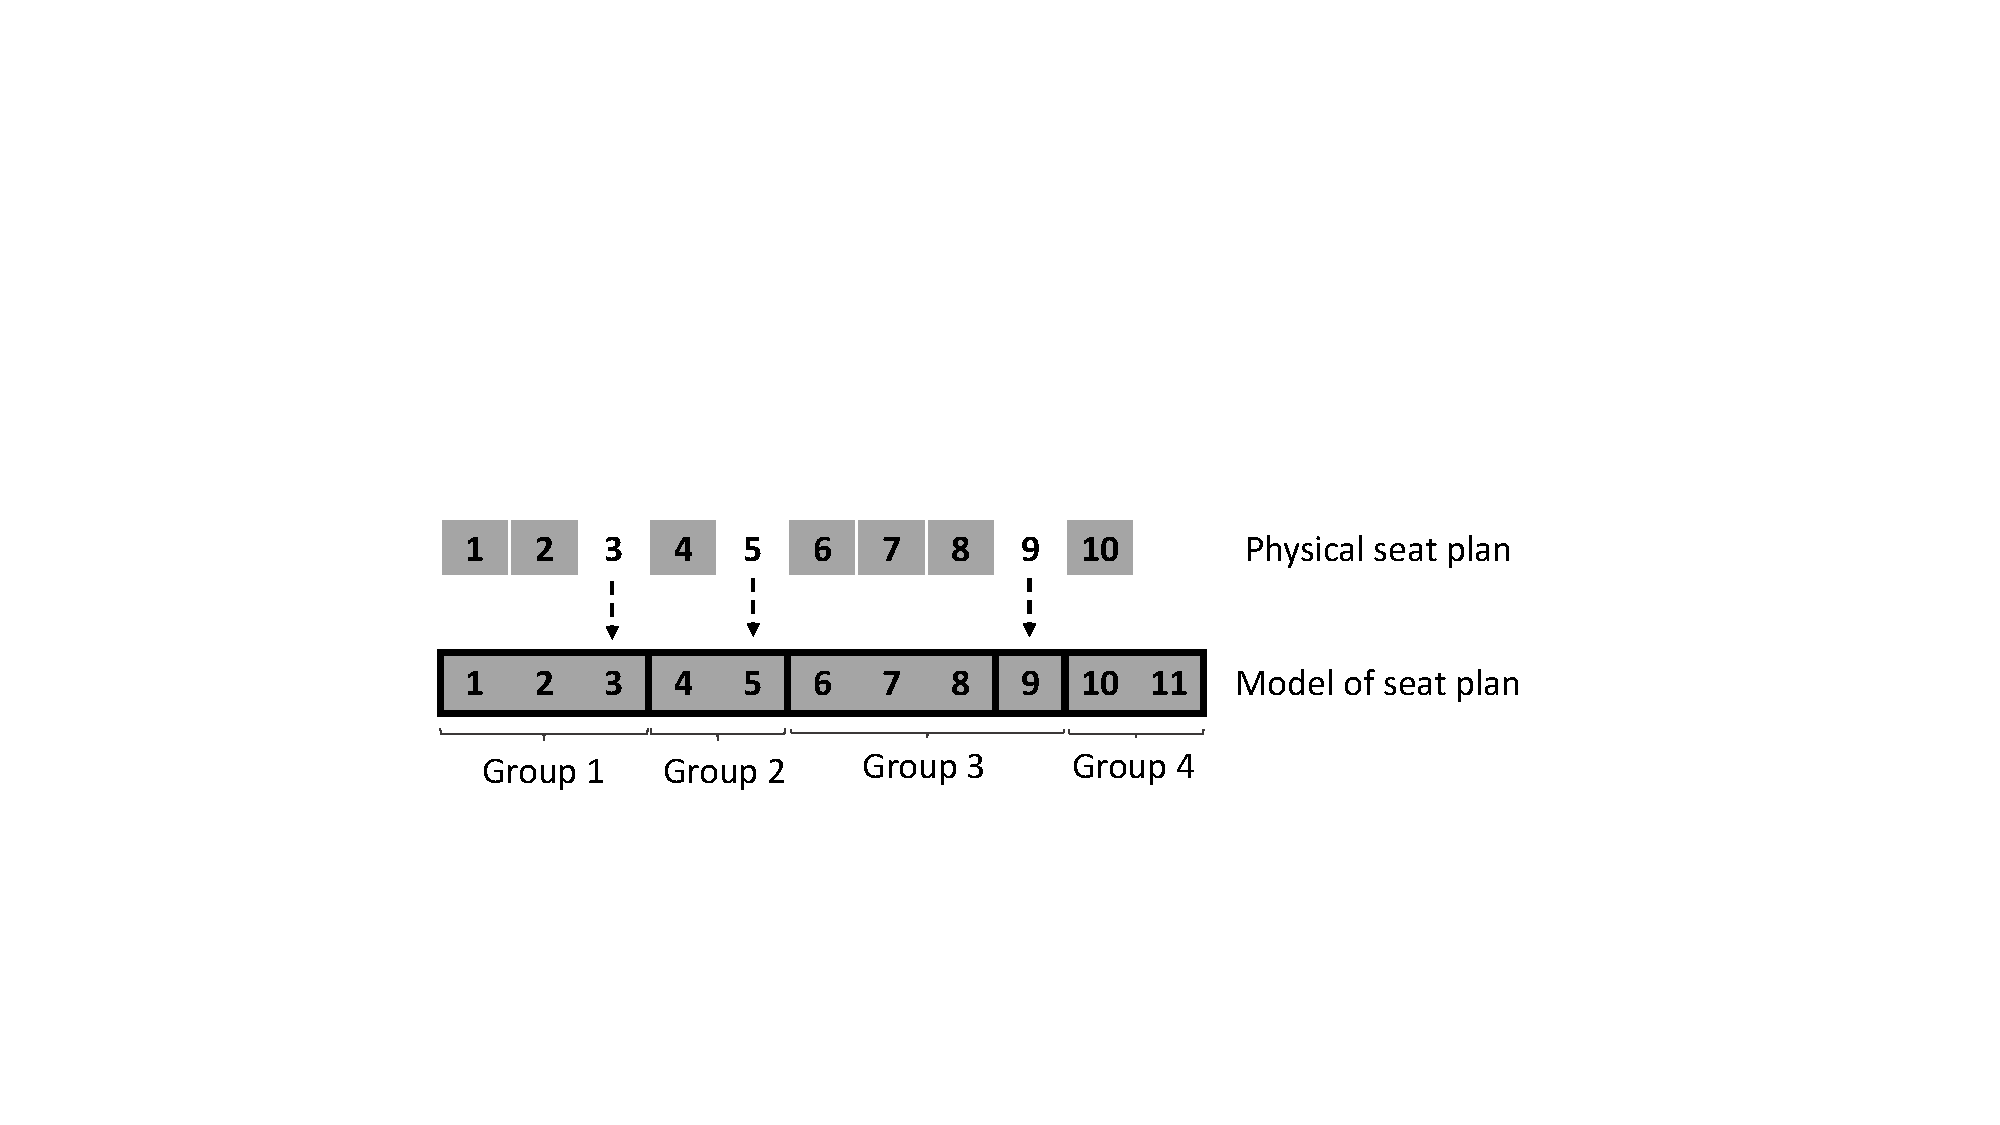
\includegraphics[width=0.55\textwidth]{./Figures/model_plan.pdf}
\end{figure}

We now formulate the seat planning with deterministic requests (SPDR) problem as an integer programming, where $x_{ij}$ represents the number of groups of type $i$ planned in row $j$. 

\begin{align}
(\text{SPDR}) \quad \max \quad & \sum_{i=1}^{M}  \sum_{j= 1}^{N} (n_i - \delta) x_{ij} \label{e0} \\
\text {s.t.} \quad & \sum_{j= 1}^{N} x_{ij} \leq d_{i}, \quad i \in \mathcal{M}, \label{deter_upper}\\ 
& \sum_{i=1}^{M} n_{i} x_{ij} \leq L_j, j \in \mathcal{N}, \label{capa_con} \\
& x_{ij} \in \mathbb{N}, \quad i \in \mathcal{M}, j \in \mathcal{N}. \notag 
\end{align}


The objective function (\ref{e0}) is to maximize the number of individuals accommodated. Constraint \eqref{deter_upper} ensures the total number of accommodated groups does not exceed the number of requests for each group type. Constraint \eqref{capa_con} stipulates that the number of seats allocated in each row does not exceed the size of the row.

The increasing nature of the ratio $\frac{i}{n_i}$ with respect to group size $i$ leads to preferential inclusion of larger groups in the optimal fractional seat plan. This intuitive property is illustrated in Proposition \ref{sol_relax_deter}. 

% By examining the monotonic ratio of $\frac{i}{n_i}$, we can establish the upper bound of supply corresponding to the optimal solution of the LP relaxation of SPDR problem.


% and will be utilized in the bid-price control policy discussed in Section \ref{bid_price}.

\begin{prop}\label{sol_relax_deter}
For the LP relaxation of the \textup{SPDR} problem, there exists an index $\tilde{i}$ such that the optimal solutions satisfy the following conditions: $x_{ij}^{*} = 0$ for all $j$, $i = 1,\ldots, \tilde{i}-1$; $\sum_{j=1}^{N} x_{ij}^{*} = d_{i}$ for $i = \tilde{i}+1,\ldots, M$; $\sum_{j=1}^{N} x_{ij}^{*} = \frac{L - \sum_{i = \tilde{i}+1}^{M} {d_i n_i}}{n_{\tilde{i}}}$ for $i = \tilde{i}$.
\end{prop}

Proposition \ref{sol_relax_deter} implies that, in the optimal fractional seat plan, the requests from larger groups ($i > \tilde{i}$) are fully accommodated by the available supply. The requests from smaller groups ($i < \tilde{i}$) are rejected. Any remaining supply, if available, will be used to partially satisfy the request from group type $\tilde{i}$. The dual analysis of LP relaxation of the \textup{SPDR} problem and Proposition \ref{sol_relax_deter} will be utilized in the bid-price control policy discussed in Appendix \ref{policies}.

\subsection{Seat Planning with Full or Largest Patterns}\label{seat_planning_full_largest}
%%The seat plan obtained from \textup{SPDRP} may not utilize all available seats, as it depends on the given requests. To improve a given seat plan and utilize all seats, we aim to generate a new seat plan with full or largest patterns while ensuring that the original group type requirements are met.
While the SPDR problem is straightforward to solve for practical problems, the optimal solution reveals some interesting observations about the structure of the optimal seat plan. Specifically, when some constraints (\ref{deter_upper}) are not binding, most constraints (\ref{capa_con}) tend to be tight. In other words, in the case of supply less than demand, the seats in each row are likely to be fully used. It is worth noting that each constraint in (\ref{capa_con}) corresponds to a seating pattern of a row.
This insight leads to the following definition.

\begin{definition}
Consider a pattern $\bm{h} = (h_1, \ldots, h_M)$ for a row of size $L$. We say $\bm{h}$ to be a full pattern if $\sum_{i=1}^{M} n_i h_i = L$, and $\bm{h}$ to be a largest pattern if its size $|\bm{h}| \geq |\bm{h}^{\prime}|$, for any other feasible pattern $\bm{h}^{\prime}$.
\end{definition}

The above concepts characterize two types of tightness in a seating pattern. In a full pattern, the corresponding constraint is mathematically tight. In a maximum pattern, mathematical tightness is not enforced on the constraint; instead, it is reflected with respect to the objective function in that any other pattern cannot yield a higher objective function value. Both full pattern and maximum patterns indicate efficient  use of seats and shall be used in an optimal seat plan.


\begin{prop}\label{lem_pattern}
The size of a largest pattern, denoted by $\phi(M, L^{0}, \delta)$ as a function of $M$, $L^{0}$ and $\delta$, is given by $$\phi(M, L^{0}, \delta) = q M + \max\{r-\delta, 0\},$$ where $q$ is the quotient of $(L^{0} + \delta)$ divided by $(M+\delta)$ and $r$ is the remainder. In addition, $\phi(M, L^{0}, \delta)$ is non-decreasing in $M$ and $L^{0}$, and non-increasing in $\delta$, respectively. 
\end{prop}

The size, $qM + \max\{r-\delta, 0\}$, corresponds directly to a largest pattern which includes $q$ group type $M$ and $r$ seats allocated to a group type $(r-\delta)$ when $r>\delta$. However, the form of the largest pattern is not unique; there are other largest patterns with the same size. 
Specifically, when $r = 0$, the largest pattern is unique and full, indicating that only one pattern can accommodate the maximum number of individuals; when $r > \delta$, the largest pattern is full, as it uses all available seats. A concrete example illustrating largest and full patterns is provided in Example \ref{ex_2}. 

We can also measure the effectiveness of a seat plan by measuring the relative utilization of the seats. To this end, we define the occupancy rate of a pattern $h$ as $|h|/L^0$. By this definition, a largest pattern achieves the maximum achievable occupancy rate of a row. Similarly, we can define the maximum achievable occupancy rate of the venue as follows. 
$$\rho^{\textup{ac}} =  \frac{\sum_{j =1}^{N}\phi(M, L_{j}^{0}, \delta)}{\sum_{j =1}^{N} L_{j}^{0}},$$
where $\phi(M, L^{0}, \delta)$ represents the size of the largest pattern under $M$, $L^{0}$ and $\delta$.

The monotonicity of $\phi(M, L^{0}, \delta)$ stated in Proposition \ref{lem_pattern} also applies to the maximum achievable occupancy rate with respect to $M$ and $\delta$, but not with respect to $L^{0}$. This result is established in the following corollary. 
Further discussion on the maximum achievable occupancy rate will be provided in Section \ref{impact_sd}.


\begin{corollary}\label{maximum_phi}
The maximum achievable occupancy rate is non-decreasing in $M$ and non-increasing in $\delta$, but not monotone in $L_{j}^{0}, \forall j \in \mathcal{N}$.
\end{corollary}

 %Similarly, the maximum achievable occupancy rate does not decrease when $\delta$ increases. Although $\phi(M, L^{0}, \delta)$ is non-decreasing in $L$, for a single row, when $L$ increases while $M$ remains unchanged, the maximum achievable occupancy rate may either increase or decrease. Consequently, the trend of the maximum achievable occupancy rate for a layout is not straightforward. 
 

\begin{example}\label{ex_2}
Consider the given values: $\delta = 1$, $L = 21$, and $M = 4$. The size of the largest pattern can be calculated as $qM + \max\{r-\delta, 0\} = 4 \times 4 + 0 = 16$. The largest patterns are as follows: $(1, 0, 1, 3)$, $(0, 1, 2, 2)$, $(0, 0, 0, 4)$, $(0, 0, 4, 1)$, and $(0, 2, 0, 3)$. Among these, $(0, 0, 0, 4)$ is the form referenced in Proposition \ref{lem_pattern}.

Figure \ref{full_largest} shows that the largest pattern may not be full and the full pattern may not be largest.
\begin{figure}[ht]
    \caption{Largest and full patterns}\label{full_largest}
    \centering
        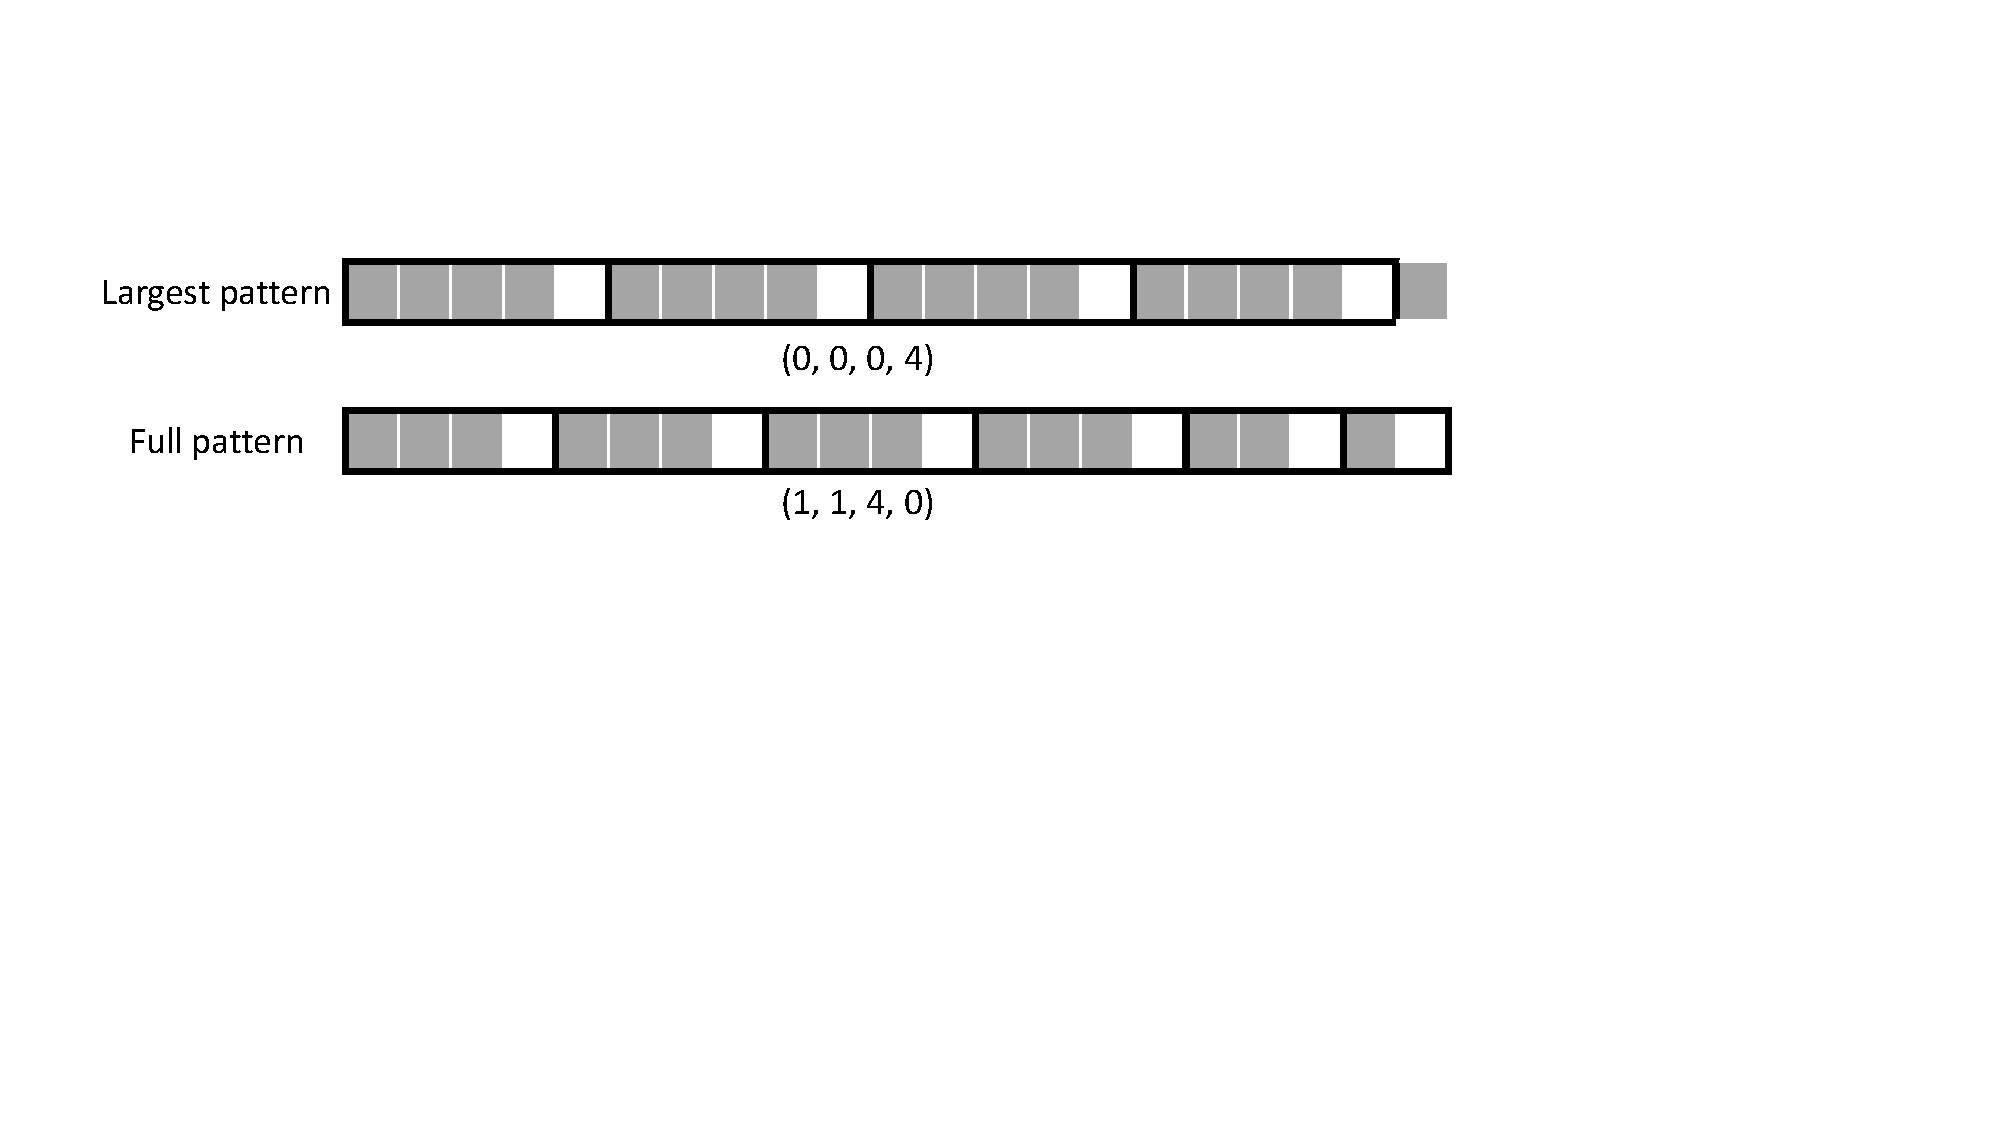
\includegraphics[width=0.8\textwidth]{./Figures/largest_full.pdf}
\end{figure}

Pattern $(0, 0, 0, 4)$ is a largest pattern as its size is 16. However, it does not satisfy the requirement of fully utilizing all available seats since $4 \times 5 \neq 21$. Pattern $(1, 1, 4, 0)$ is a full pattern as it utilizes all available seats. However, its size is 15, indicating that it is not a largest pattern.
\end{example}

%When the constraints \eqref{deter_upper} are tight while most constraints \eqref{capa_con} remain loose, indicating the availability of many seats, our goal 

 Given a feasible seat plan, our goal is to derive a seat plan that satisfies the original requirements of the feasible seat plan while utilizing as many seats as possible. Will the optimal seat plan consist of either full or largest patterns? To address this question, let the feasible seat plan be $\bm{H}$ and the desired seat plan be $\bm{H}^{\prime}$. To satisfy the requirements of planned group types in $\bm{H}$, the total quantity of groups from type $i$ to type $M$ in $\bm{H}^{\prime}$ must be at least equal to the total quantity from group type $i$ to group type $M$ in $\bm{H}$. Mathematically, we aim to find a feasible seat plan $\bm{H}^{\prime}$ such that $\sum_{k=i}^{M} \sum_{j=1}^{N} H_{kj} \leq \sum_{k=i}^{M} \sum_{j=1}^{N} H^{\prime}_{kj}, \forall i \in \mathcal{M}$. We say $\bm{H} \subseteq \bm{H}^{\prime}$ if this condition is satisfied.

To utilize all seats in the seat plan, the objective is to maximize the number of individuals that can be accommodated. Thus, we have the following formulation:

\begin{equation}\label{improve_seat}
  \begin{aligned}
  \max \quad & \sum_{i=1}^{M} \sum_{j=1}^{N} (n_i-\delta)  x_{ij} \\
  s.t. \quad & \sum_{k=i}^{M} \sum_{j=1}^{N}  x_{kj} \geq  \sum_{k=i}^{M} \sum_{j=1}^{N} H_{kj}, i \in \mathcal{M} \\
  & \sum_{i=1}^{M} n_{i} x_{ij} \leq L_{j}, j \in \mathcal{N} \\
  & x_{ij} \in \mathbb{N}, i \in \mathcal{M}, j \in \mathcal{N}
  \end{aligned}
\end{equation}

\begin{prop}\label{prop_construction}
Given a feasible seat plan $\bm{H}$, the optimal solution to problem \eqref{improve_seat} corresponds to a seat plan $\bm{H}^{\prime}$ such that $\bm{H} \subseteq \bm{H}^{\prime}$ and $\bm{H}^{\prime}$ is composed of either full or largest patterns.
\end{prop}


This approach guarantees the seat allocation with full or largest patterns while still accommodating the original groups' requirements. Furthermore, the improved seat plan can be used for the seat assignment when the group arrives sequentially.

